%%%%%%%%%%%%%%%%%%%%%%%%%%%%%%%%%%%%%%%%%
% Beamer Presentation
% LaTeX Template
% Version 1.0 (10/11/12)
%
% This template has been downloaded from:
% http://www.LaTeXTemplates.com
%
% License:
% CC BY-NC-SA 3.0 (http://creativecommons.org/licenses/by-nc-sa/3.0/)
%
%%%%%%%%%%%%%%%%%%%%%%%%%%%%%%%%%%%%%%%%%

%----------------------------------------------------------------------------------------
%	PACKAGES AND THEMES
%----------------------------------------------------------------------------------------

\documentclass[hyperref={colorlinks=true,pdfpagelabels=false,linkcolor=black}, xcolor=dvipsnames,10pt]{beamer}
\hypersetup{pdftex=true, colorlinks=true, breaklinks=true, linkcolor=black, menucolor=blue, pagecolor=blue, urlcolor=cyan}


\usepackage{graphicx} % Allows including images
\usepackage{booktabs} % Allows the use of \toprule, \midrule and \bottomrule in tables
\usepackage{xcolor, color}% ,colortbl}
\usepackage{tikz} % nalipour
\usetikzlibrary{tikzmark} % nalipour
\usepackage{hyperref}
\usetikzlibrary{shapes,arrows, decorations.pathreplacing} %nilou
\usetikzlibrary{decorations.markings} %nilou
\usetikzlibrary{trees}%nilou
\usetikzlibrary{decorations.pathmorphing}%nilou
\usepackage{siunitx}%nilou
\usepackage{framed}%nilou
\usetikzlibrary{backgrounds} %nilou
\usepackage[framemethod=tikz]{mdframed}%nilou
\usepackage{adjustbox} %nilou for adjusting the table
\usepackage{amssymb} %nalipour for checkmark
\usepackage{libertine} % For the font

\usepackage{../../../CLICdp_definitions} % nalipour
\usepackage{xspace}
\usepackage{upgreek} % nalipour
\usepackage{amsmath, mathtools} % nalipour
\renewcommand{\thefootnote}{\fnsymbol{footnote}} % nalipour: symbols
                                % for the footnote
\usepackage{verbatim} % nalipour
\usepackage{fixltx2e}
\usepackage{adjustbox}%nalipour
\usepackage{pifont} %nalipour
\usepackage{smartdiagram}
\usesmartdiagramlibrary{additions}
\usepackage{siunitx}

\usetikzlibrary{angles,quotes}
\usetikzlibrary{positioning}

%%%%%%%%%%%%%%%%%%%%%%%%%%%%%

%----------------------------------------------------------------------------------------
%	TITLE PAGE
%----------------------------------------------------------------------------------------
\title[]{Full simulation of the FCC-ee IDEA detector with FCCSW}
\author[Niloufar Alipour Tehrani]{Niloufar Alipour Tehrani
  \vspace{0.3cm} }

\institute[CERN]{}
\date[6 July 2018]{RD-FA Collaboration Meeting\\ \vspace{0.3cm}
  \scriptsize{CERN \\
6 July 2018}}


\setbeamertemplate{navigation symbols}{}
\setbeamertemplate{footline}[frame number]

\usetheme{default}%CambridgeUS}%Boadilla}%Pittsburgh}
\usecolortheme{default}

\setlength{\leftmargini}{2pt} % nalipour: left margin indentation
\renewcommand{\inserttotalframenumber}{\ref{lastframe}}
\begin{document}
\renewcommand{\inserttotalframenumber}{\pageref{lastslide}}

\tikzset{cross/.style={cross out, draw=black, minimum
    size=2*(#1-\pgflinewidth), inner sep=0pt, outer sep=0pt}, %default
  radius will be 1pt.  cross/.default={1pt}}


%%%%%%%%%%%%%%%%%%%%%%%%%%%%%
%         SLIDE             %
%%%%%%%%%%%%%%%%%%%%%%%%%%%%%
\begin{frame}[plain]

  \titlepage
  \begin{columns}
    \column{0.25\textwidth}
    \centering
    
\includegraphics[width=\textwidth]{../../../logos/FCC-logo}
    \column{0.5\textwidth}
    \column{0.25\textwidth}
    \centering
    
\includegraphics[width=0.6\textwidth]{../../../logos/logo_cern.pdf}
  \end{columns}
\end{frame}

%%%%%%%%%%%%%%%%%%%%%%%%%%%%%
%         SLIDE             %
%%%%%%%%%%%%%%%%%%%%%%%%%%%%%
\begin{frame}
\frametitle{FCC Software: FCCSW}

  \begin{columns}
  \column{0.5\textwidth}
  \begin{itemize}
  \item Common software for all FCC experiments
    \begin{itemize}
    \item ee, hh \& eh \vspace{0.5cm}
    \end{itemize}
  \item Detector and physics studies
    \begin{itemize}
    \item Fast \& full simulations
    \item One software stack from event generation to
                  physics analysis \vspace{0.5cm}
    \end{itemize}
  \item Collaborative approach
    \begin{itemize}
    \item LHC: Gaudi
    \item CLIC: DD4hep
    \item New solutions $\Rightarrow$ where needed
    \end{itemize}
  \end{itemize}

  \column{0.5\textwidth}
  \centering
  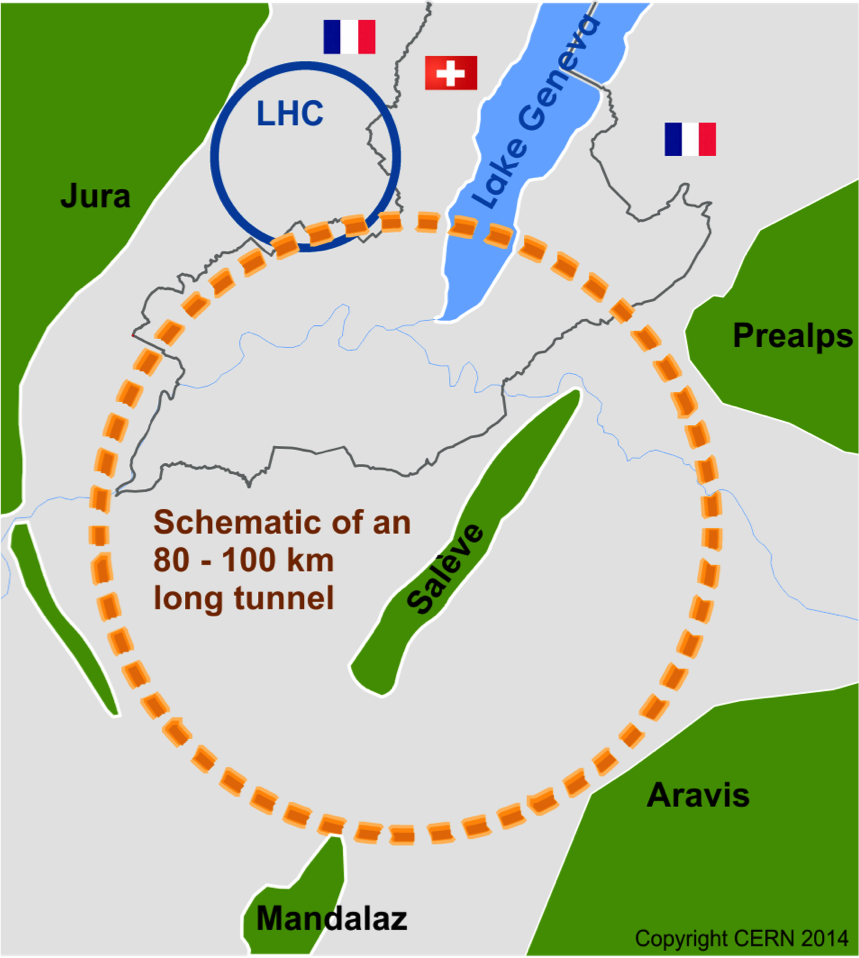
\includegraphics[width=\textwidth]{figures/cernFCC}
  \end{columns}

  \vspace{0.5cm}
  \begin{itemize}
    \item The IDEA concept is under development within FCCSW
      \begin{itemize}
        \item Impact of beam-induced background is under study
      \end{itemize}
  \end{itemize}

\end{frame}

%%%%%%%%%%%%%%%%%%%%%%%%%%%%%
%         SLIDE             %
%%%%%%%%%%%%%%%%%%%%%%%%%%%%%
\begin{frame}
	\frametitle{FCCSW}

    \begin{itemize}
      \item Webpage and tutorials: \url{http://fccsw.web.cern.ch/fccsw}
      \item GitHub link for the code: \url{https://github.com/HEP-FCC/FCCSW}
    \end{itemize}

    \centering
		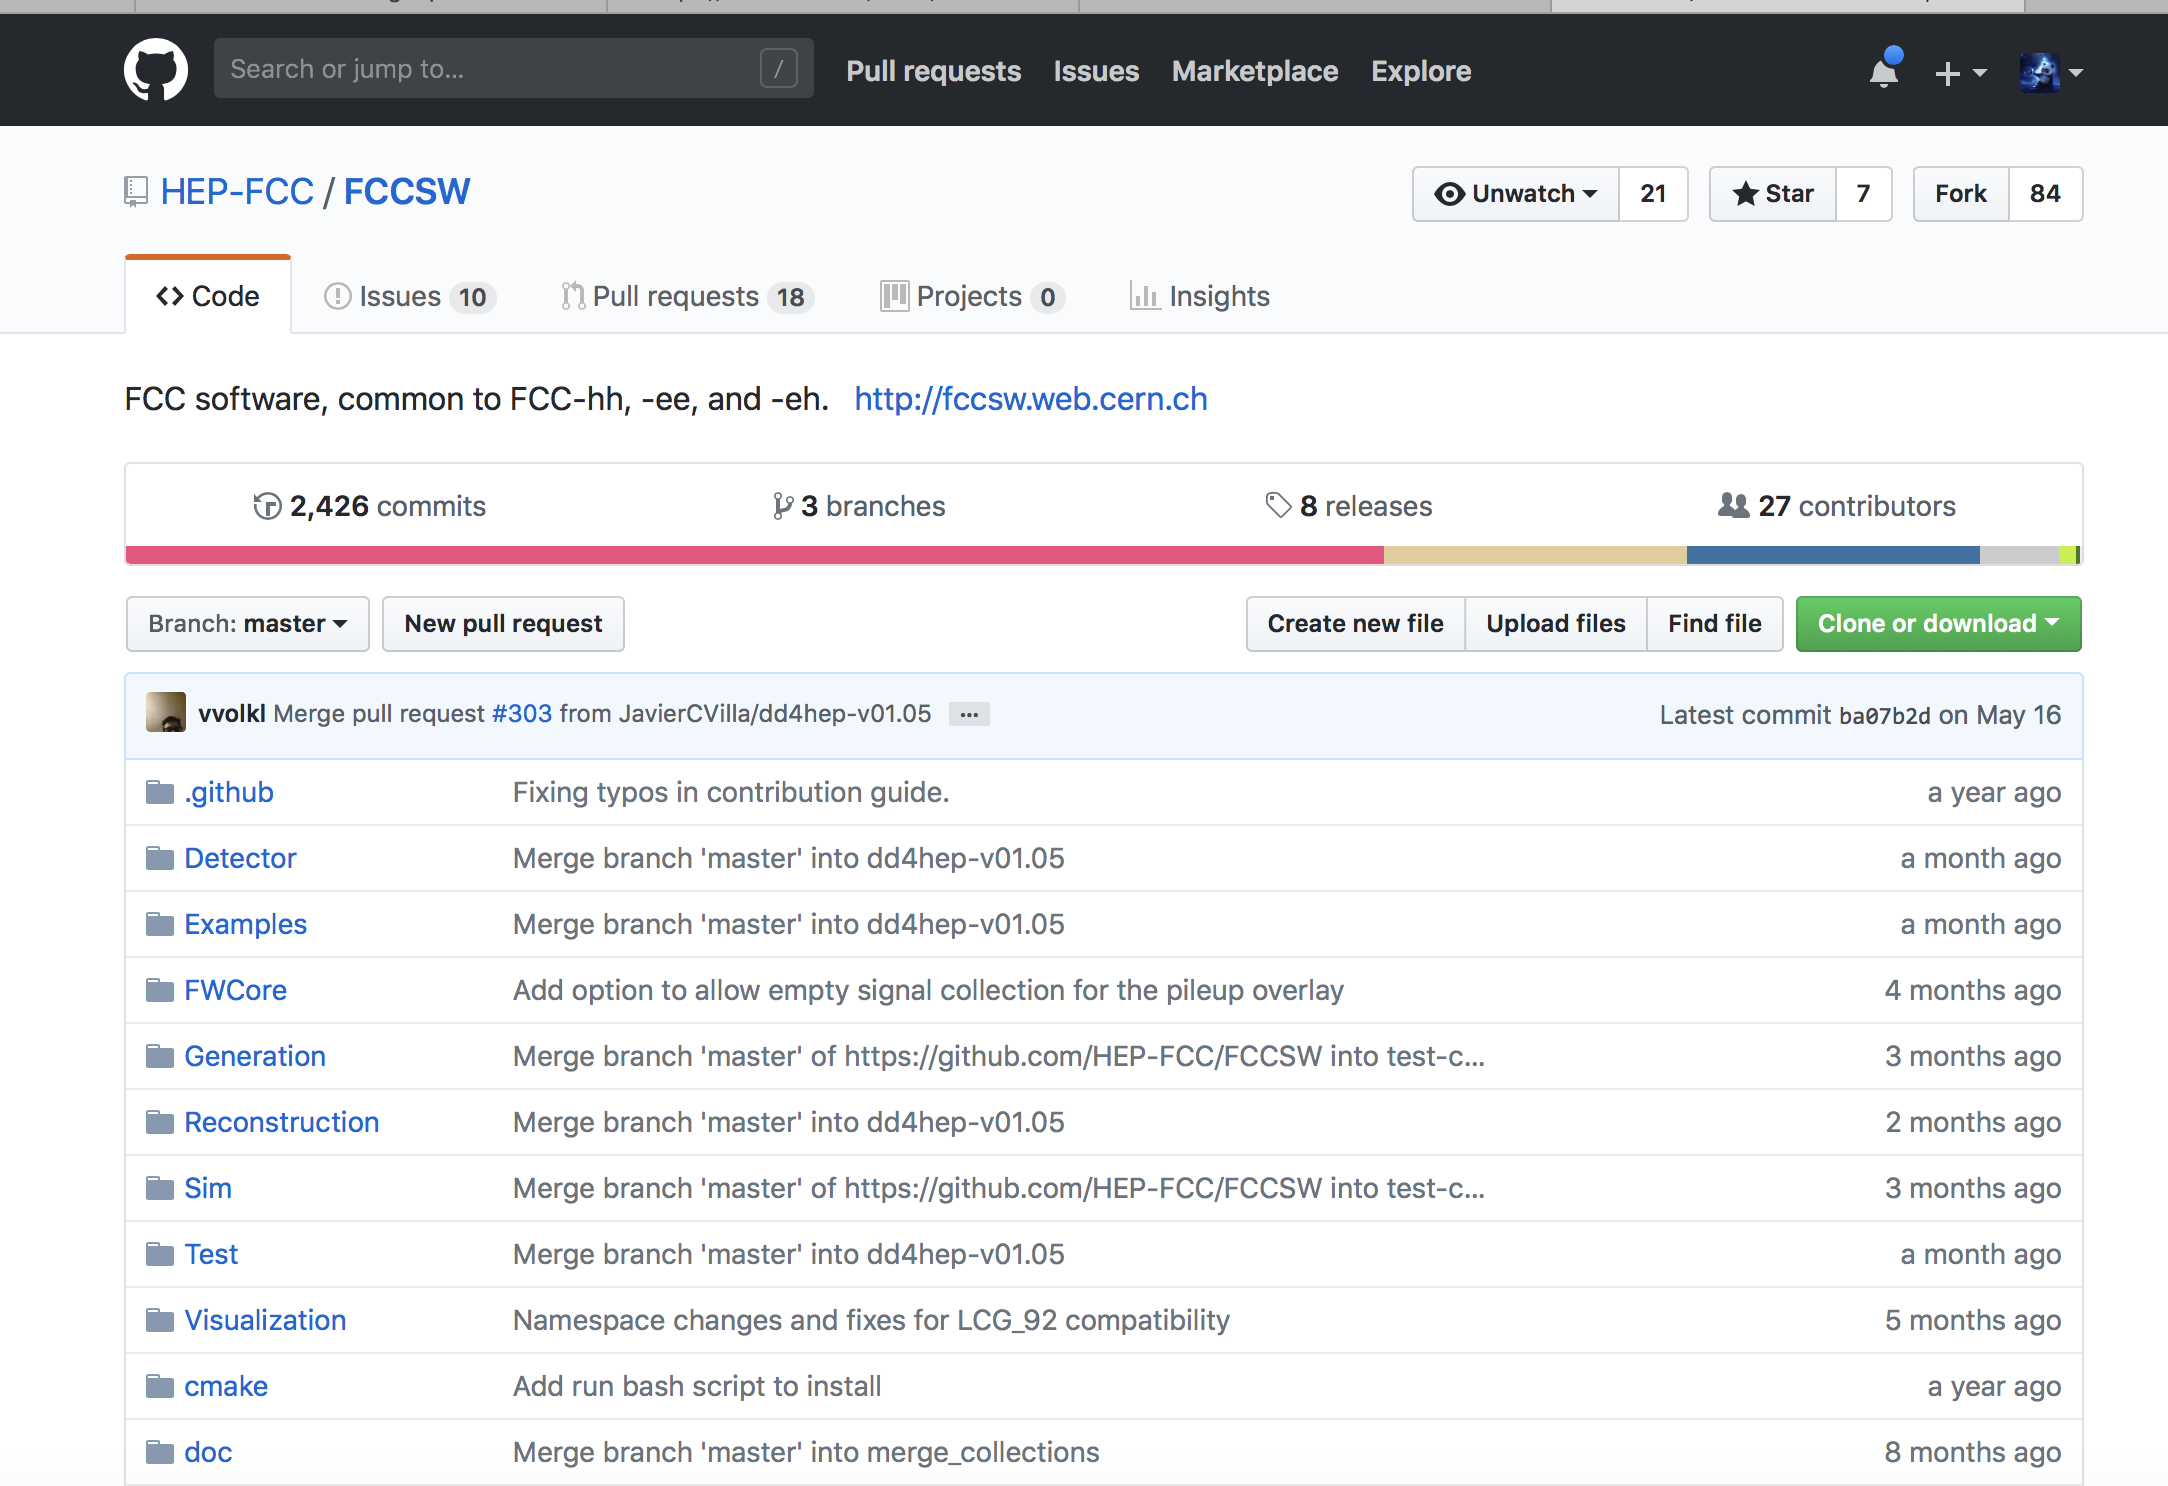
\includegraphics[width=\textwidth]{./figures/GitHub}
\end{frame}


%%%%%%%%%%%%%%%%%%%%%%%%%%%%%
%         SLIDE             %
%%%%%%%%%%%%%%%%%%%%%%%%%%%%%
\begin{frame}
	\frametitle{The IDEA interaction region in FCCSW}

	\begin{itemize}
	\item Beam-pipe, beam instrumentations and the vertex detector are taken from the CLD concept
		\begin{itemize}
		\item Temporary design of VXD for the IDEA detector $\Rightarrow $ ultimate goal: MAPS
		\end{itemize}
	\item The DCH implemented from scratch in FCCSW
  \item Missing elements
    \begin{itemize}
      \item Alice-like ITS, solenoid magnet, dual-readout calorimeter, instrumented return yoke
    \end{itemize}
	\end{itemize}

  \vspace{-0.2cm}
	\begin{block}{Visualisation with FCCSW}
	\centering
	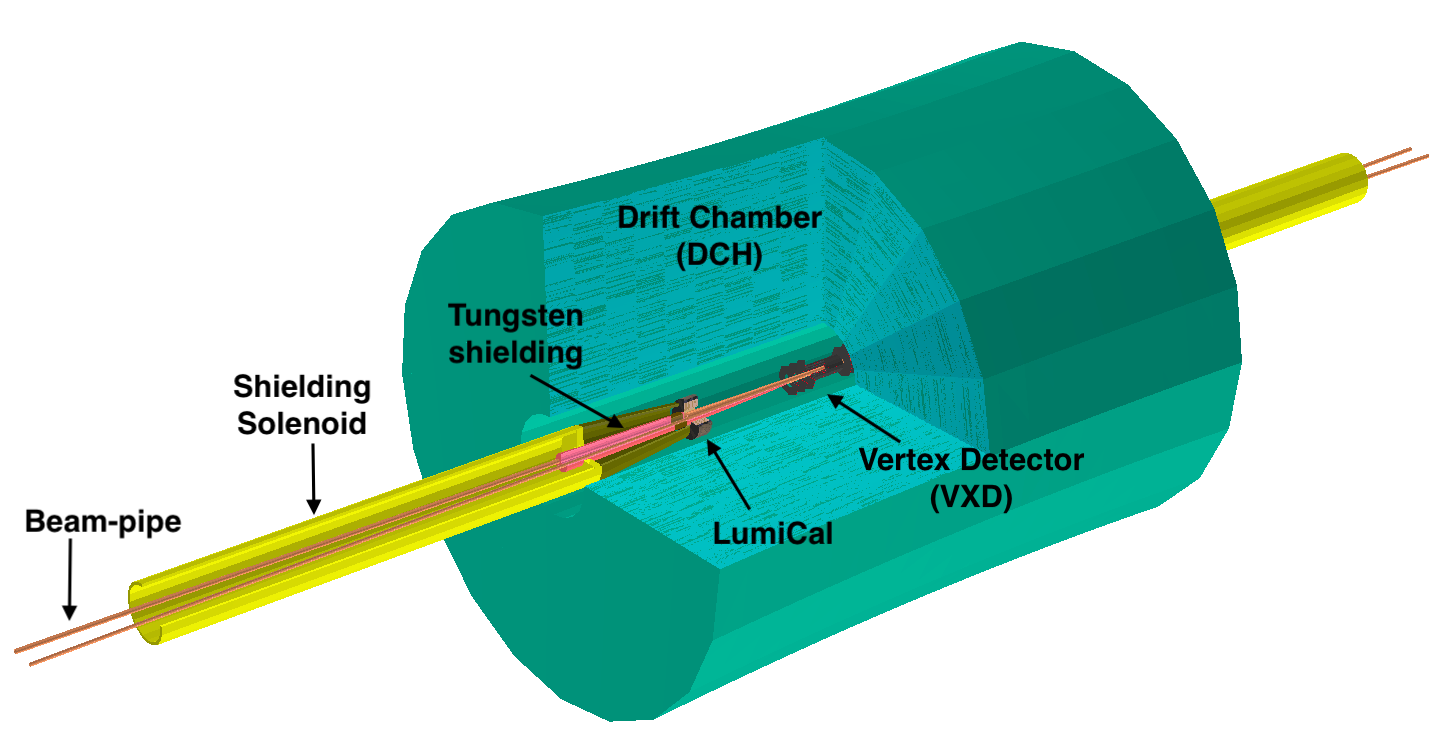
\includegraphics[width=\textwidth]{figures/FCCeeIDEA.png}
	\end{block}

\end{frame}

%%%%%%%%%%%%%%%%%%%%%%%%%%%%%
%         SLIDE             %
%%%%%%%%%%%%%%%%%%%%%%%%%%%%%
\begin{frame}
	\frametitle{FCCSW simulation chain}

	\begin{enumerate}
	\item Detector geometry description with DD4hep \vspace{0.2cm}
	\item Segmentation of the sensitive areas: \vspace{0.2cm}
		\begin{itemize}
    \item Speed up the simulation
		\item Example: information on the position of the sense wires instead of placing physical volumes \vspace{0.2cm}
		\end{itemize}
	\item Geant4 simulation: \vspace{0.2cm}
		\begin{itemize}
		\item Calculate the E\textsubscript{dep} in sensitive volumes \vspace{0.2cm}
		\end{itemize}
	\item Hit reconstruction: \vspace{0.2cm}
		\begin{itemize}
		\item Combination of individual hit calculations from (3)
		\item Calculation of the drift, diffusion and signal in the wire \vspace{0.2cm}
		\end{itemize}
	\end{enumerate}

  \vspace{0.5cm}
	\centering
	\smartdiagramset{back arrow disabled=true}
  	\smartdiagram[flow diagram:horizontal]
  	{%
    	{Geometry\\DDhep}, Segmentation, {Geant4 \\simulation}, Hit Reconstruction%
  	}


\end{frame}

%%%%%%%%%%%%%%%%%%%%%%%%%%%%%
%         SLIDE             %
%%%%%%%%%%%%%%%%%%%%%%%%%%%%%
\begin{frame}
	\frametitle{The drift chamber (DCH)}

  \begin{block}{Parameters of the DCH}
    \vspace{0.5cm}
    \begin{tabular}{l l}
      \toprule
      Length & 4500~mm \\
      Inner radius & 345~mm \\
      Outer radius & 2000~mm\\
      Number of sensitive wires & 56448 \\
      Single cell resolution (transverse plane) & 0.1~mm \\
      \bottomrule
    \end{tabular}
  \end{block}

	\begin{columns}
		\column{0.5\textwidth}
		\begin{itemize}
		  \item The segmentation concept is used to access the information on the positions of the wire
		\end{itemize}

		\column{0.5\textwidth}
		\centering
		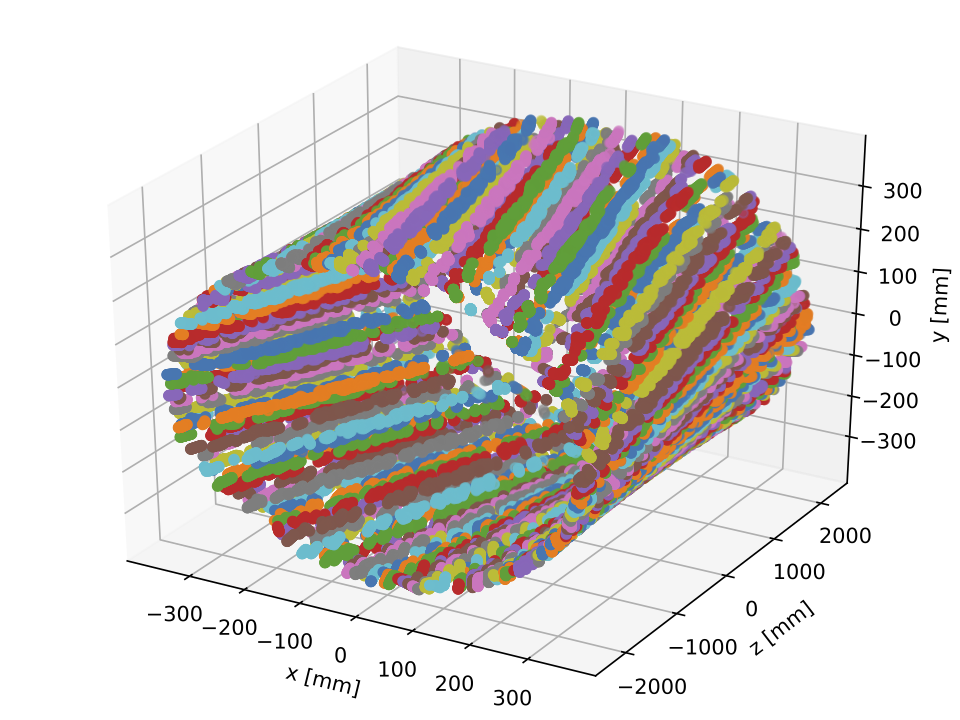
\includegraphics[width=\textwidth]{./figures/allHits}
	\end{columns}


\end{frame}


%%%%%%%%%%%%%%%%%%%%%%%%%%%%%
%         SLIDE             %
%%%%%%%%%%%%%%%%%%%%%%%%%%%%%
\begin{frame}
	\frametitle{Coverage of the drift chamber}



  \begin{columns}
    \column{0.5\textwidth}
    \begin{itemize}
      \item The number of wires as a function of $\theta$
      \item The coverage in the forward region will be improved by the placement of disks
    \end{itemize}

    \column{0.5\textwidth}
      \centering
      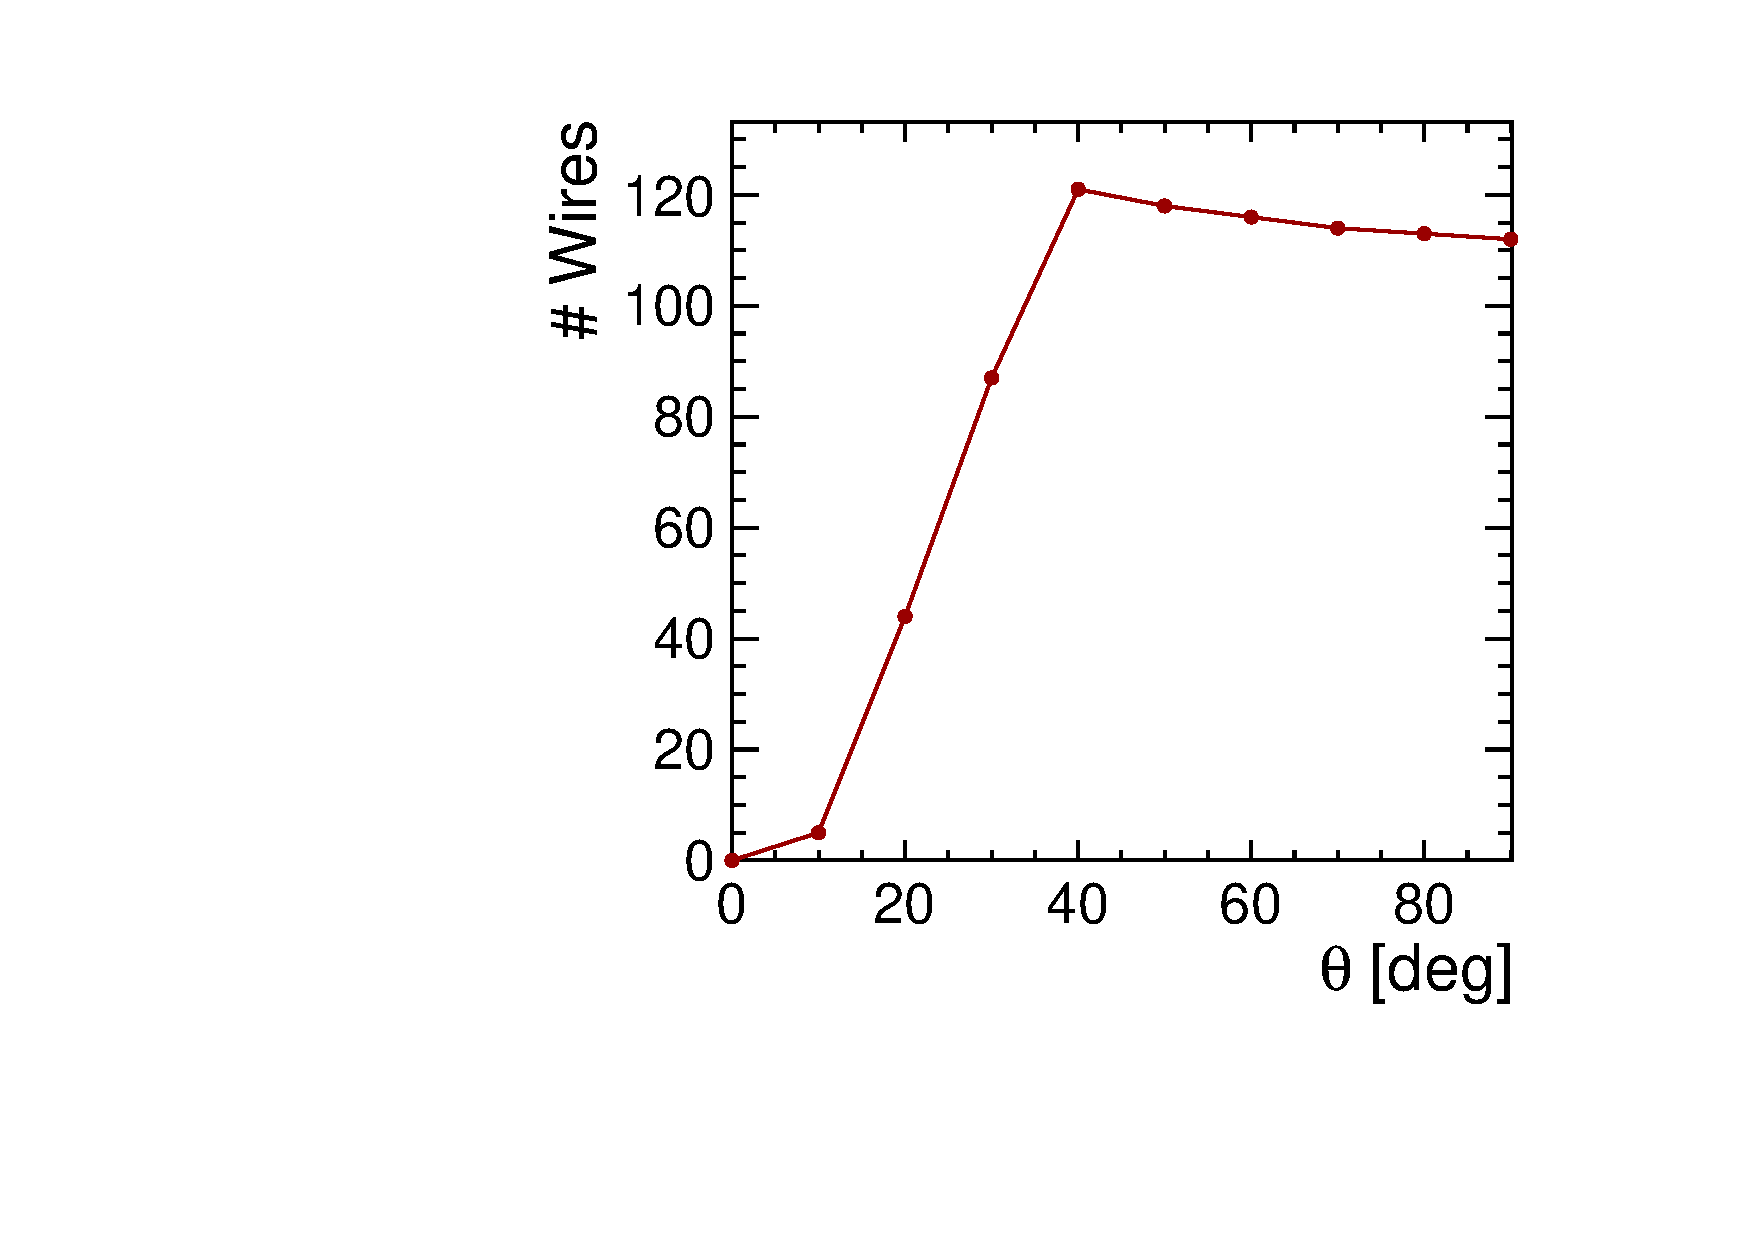
\includegraphics[width=0.9\textwidth]{./figures/numWires_theta.pdf}
  \end{columns}

  \begin{columns}
    \column{0.5\textwidth}
    \begin{itemize}
      \item The distance of the closest approach (DCA)
      \item Provides the information on the drift time
      \item Maximum drift time (corresponding to the corners): 400~ns
    \end{itemize}

    \column{0.5\textwidth}
      \centering
      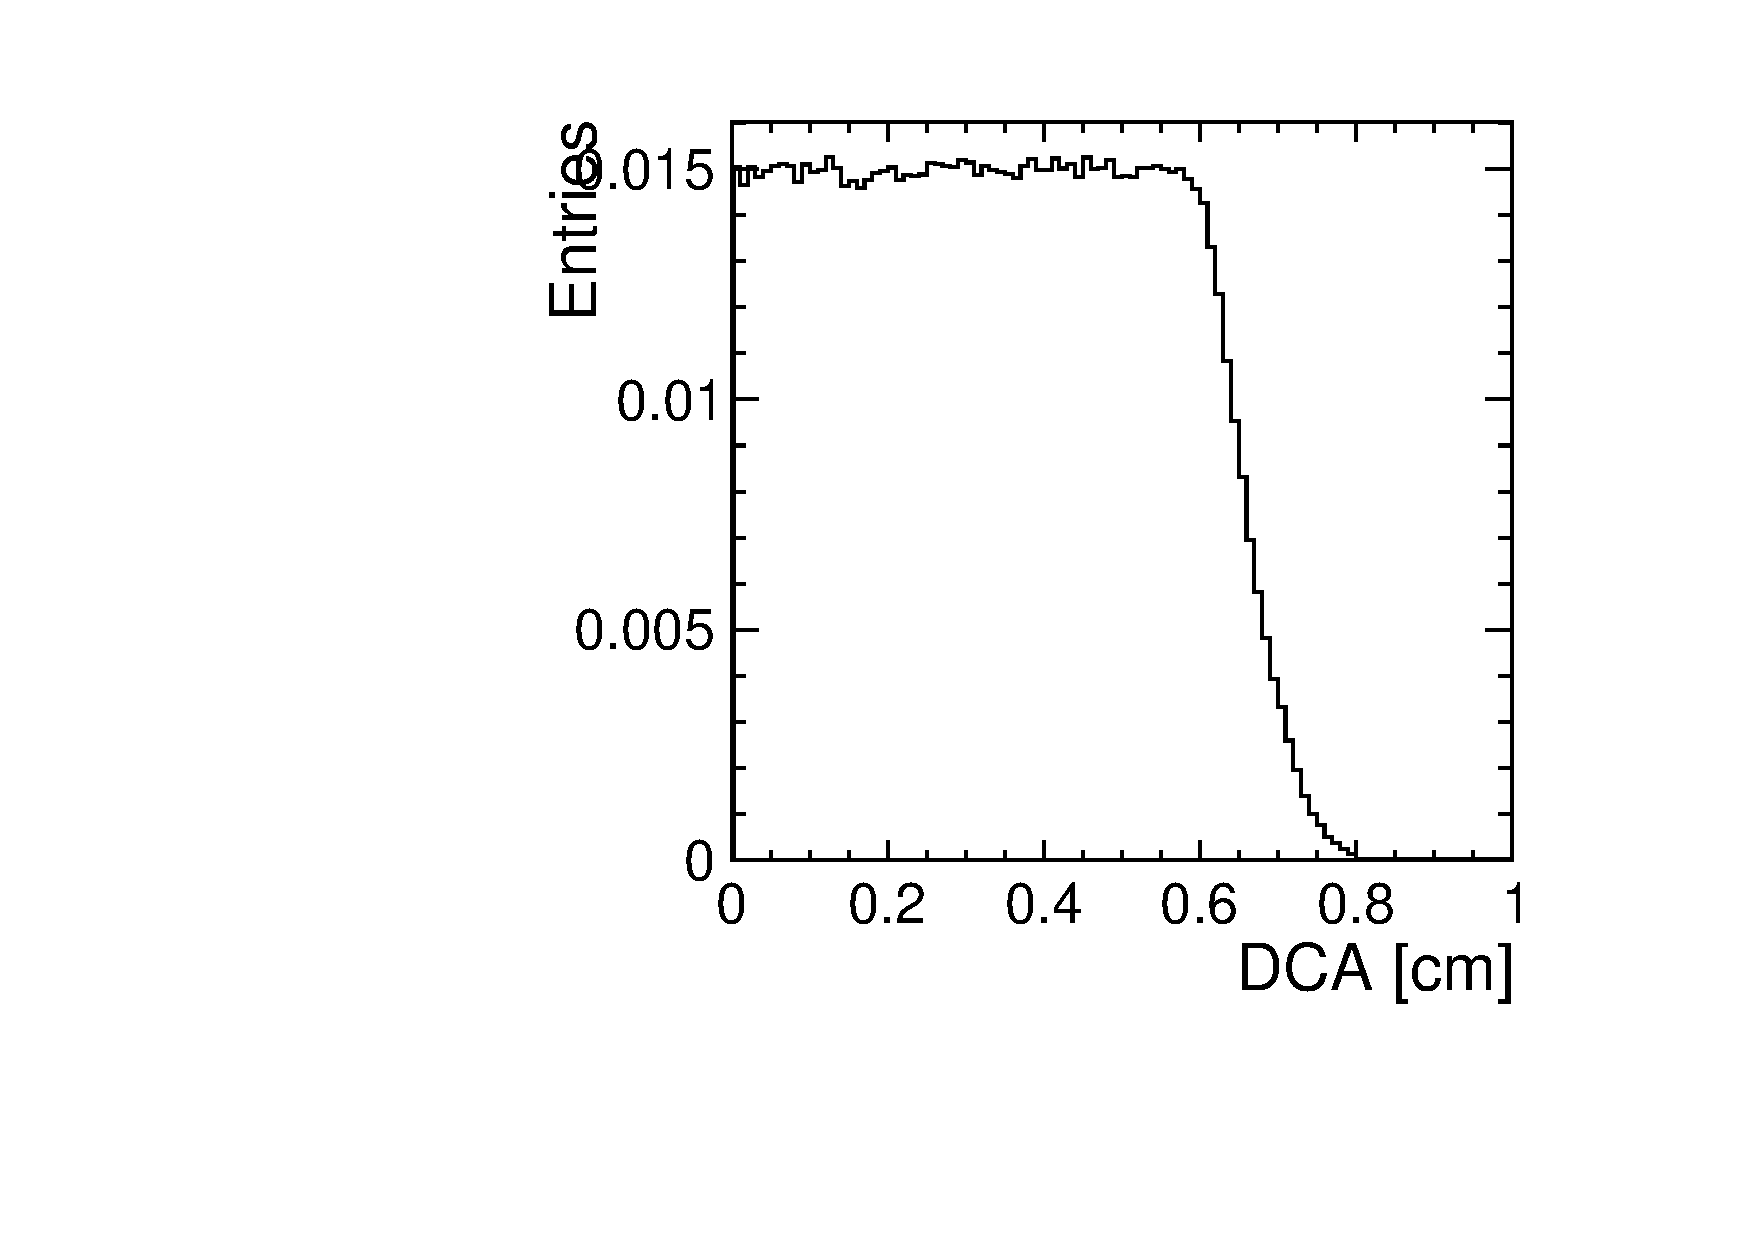
\includegraphics[width=0.9\textwidth]{./figures/DCA.pdf}
  \end{columns}

\end{frame}

%%%%%%%%%%%%%%%%%%%%%%%%%%%%%
%         SLIDE             %
%%%%%%%%%%%%%%%%%%%%%%%%%%%%%
\begin{frame}
	\frametitle{Beam-induced backgrounds at FCC-ee}

  \begin{itemize}
    \item Incoherent $e^+e^-$ pairs
      \begin{itemize}
        \item Produced in $\gamma\gamma$ interactions from beamstrahlung
        \item Forward region \vspace{0.2cm}
      \end{itemize}
    \item $\gamma\gamma\rightarrow$ hadrons
      \begin{itemize}
        \item Possibly results in jets in the detector \vspace{0.2cm}
      \end{itemize}
    \item Synchrotron radiation (SR)
      \begin{itemize}
        \item Photons from the last bending magnet
      \end{itemize}
  \end{itemize}

\end{frame}

%%%%%%%%%%%%%%%%%%%%%%%%%%%%%
%         SLIDE             %
%%%%%%%%%%%%%%%%%%%%%%%%%%%%%
\begin{frame}
	\frametitle{Incoherent $e^+e^-$ pairs}

  \begin{columns}
    \column{0.5\textwidth}
      \begin{block}{E\textsubscript{cm} = 91.2~GeV (Z stage)}
        \centering
        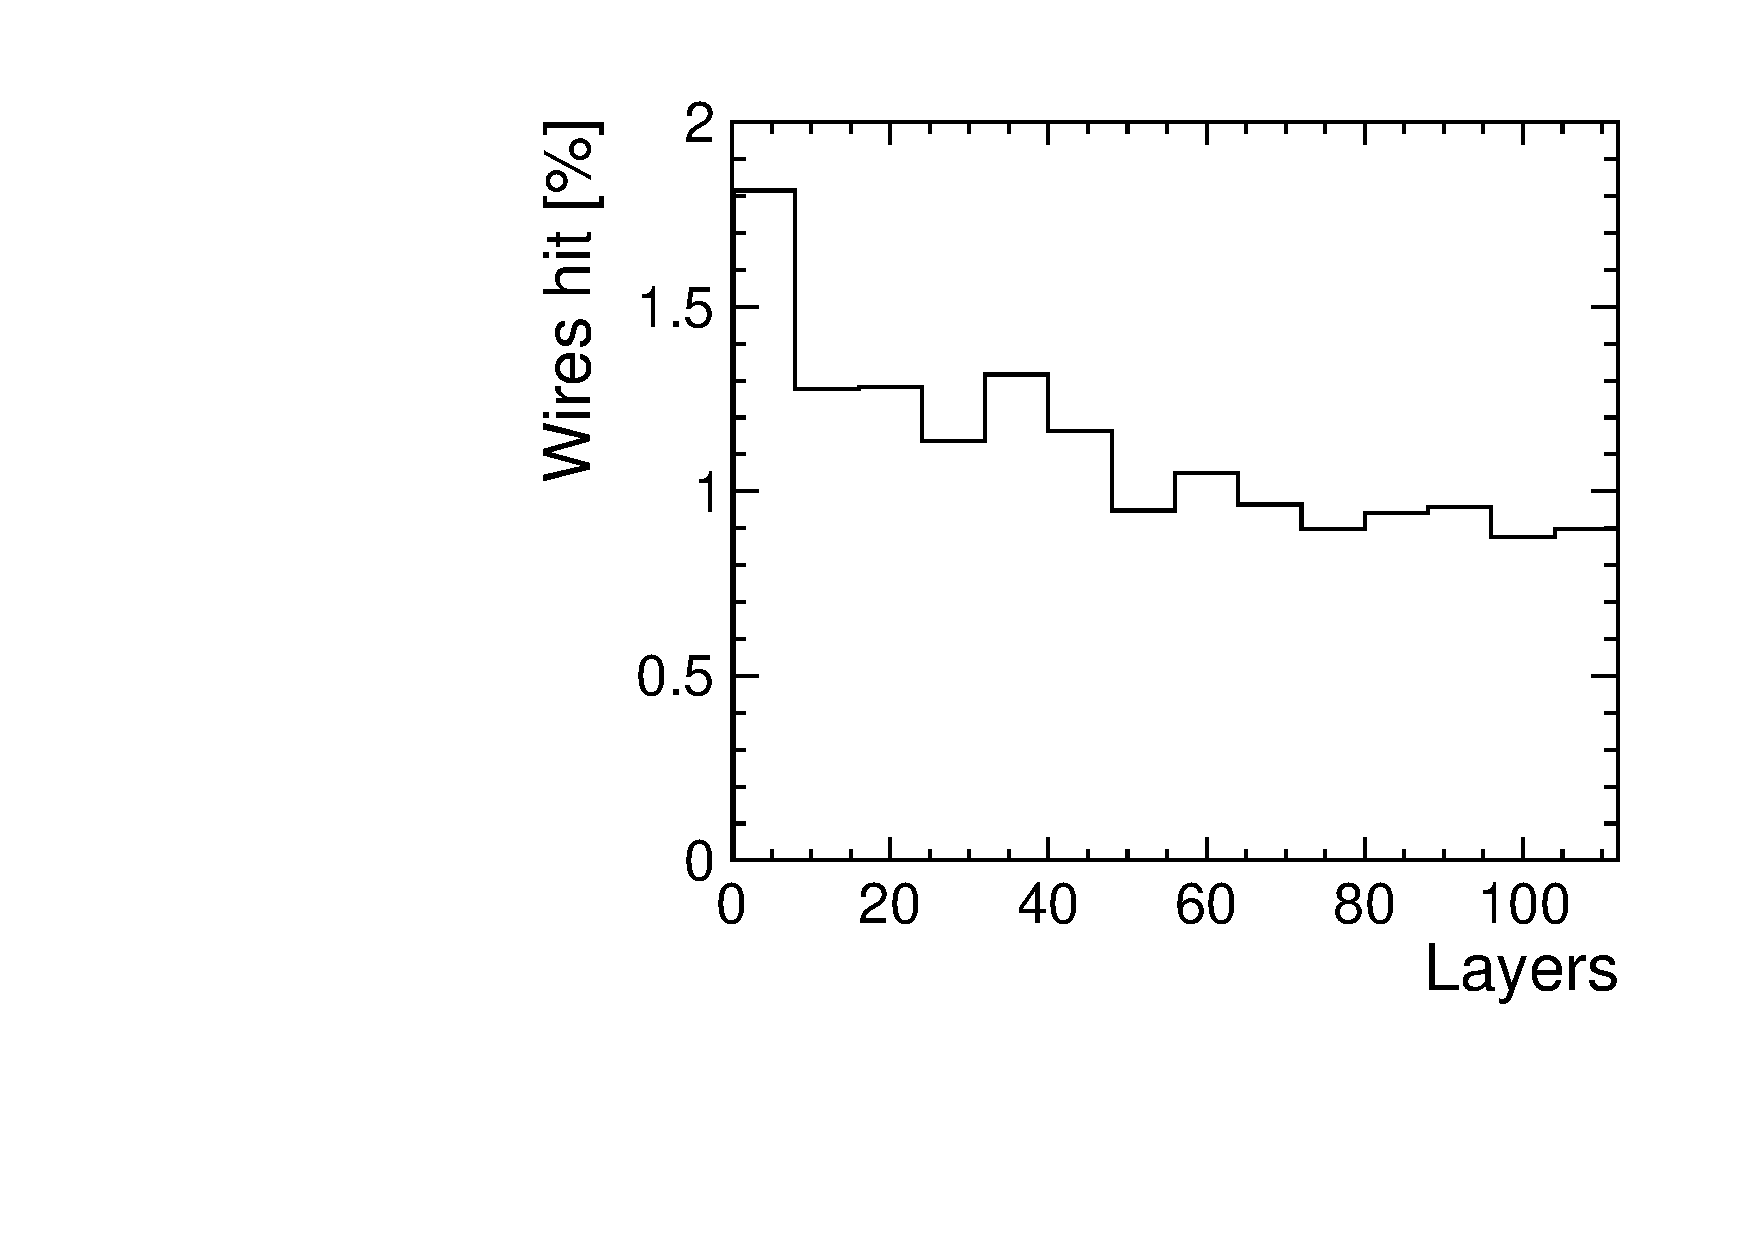
\includegraphics[width=\textwidth]{./figures/IPC_Z.pdf}
        \begin{itemize}
          \item Average occupancy: 1.1\%
        \end{itemize}
      \end{block}

    \column{0.5\textwidth}
    \begin{block}{E\textsubscript{cm} = 365~GeV (top stage)}
      \centering
      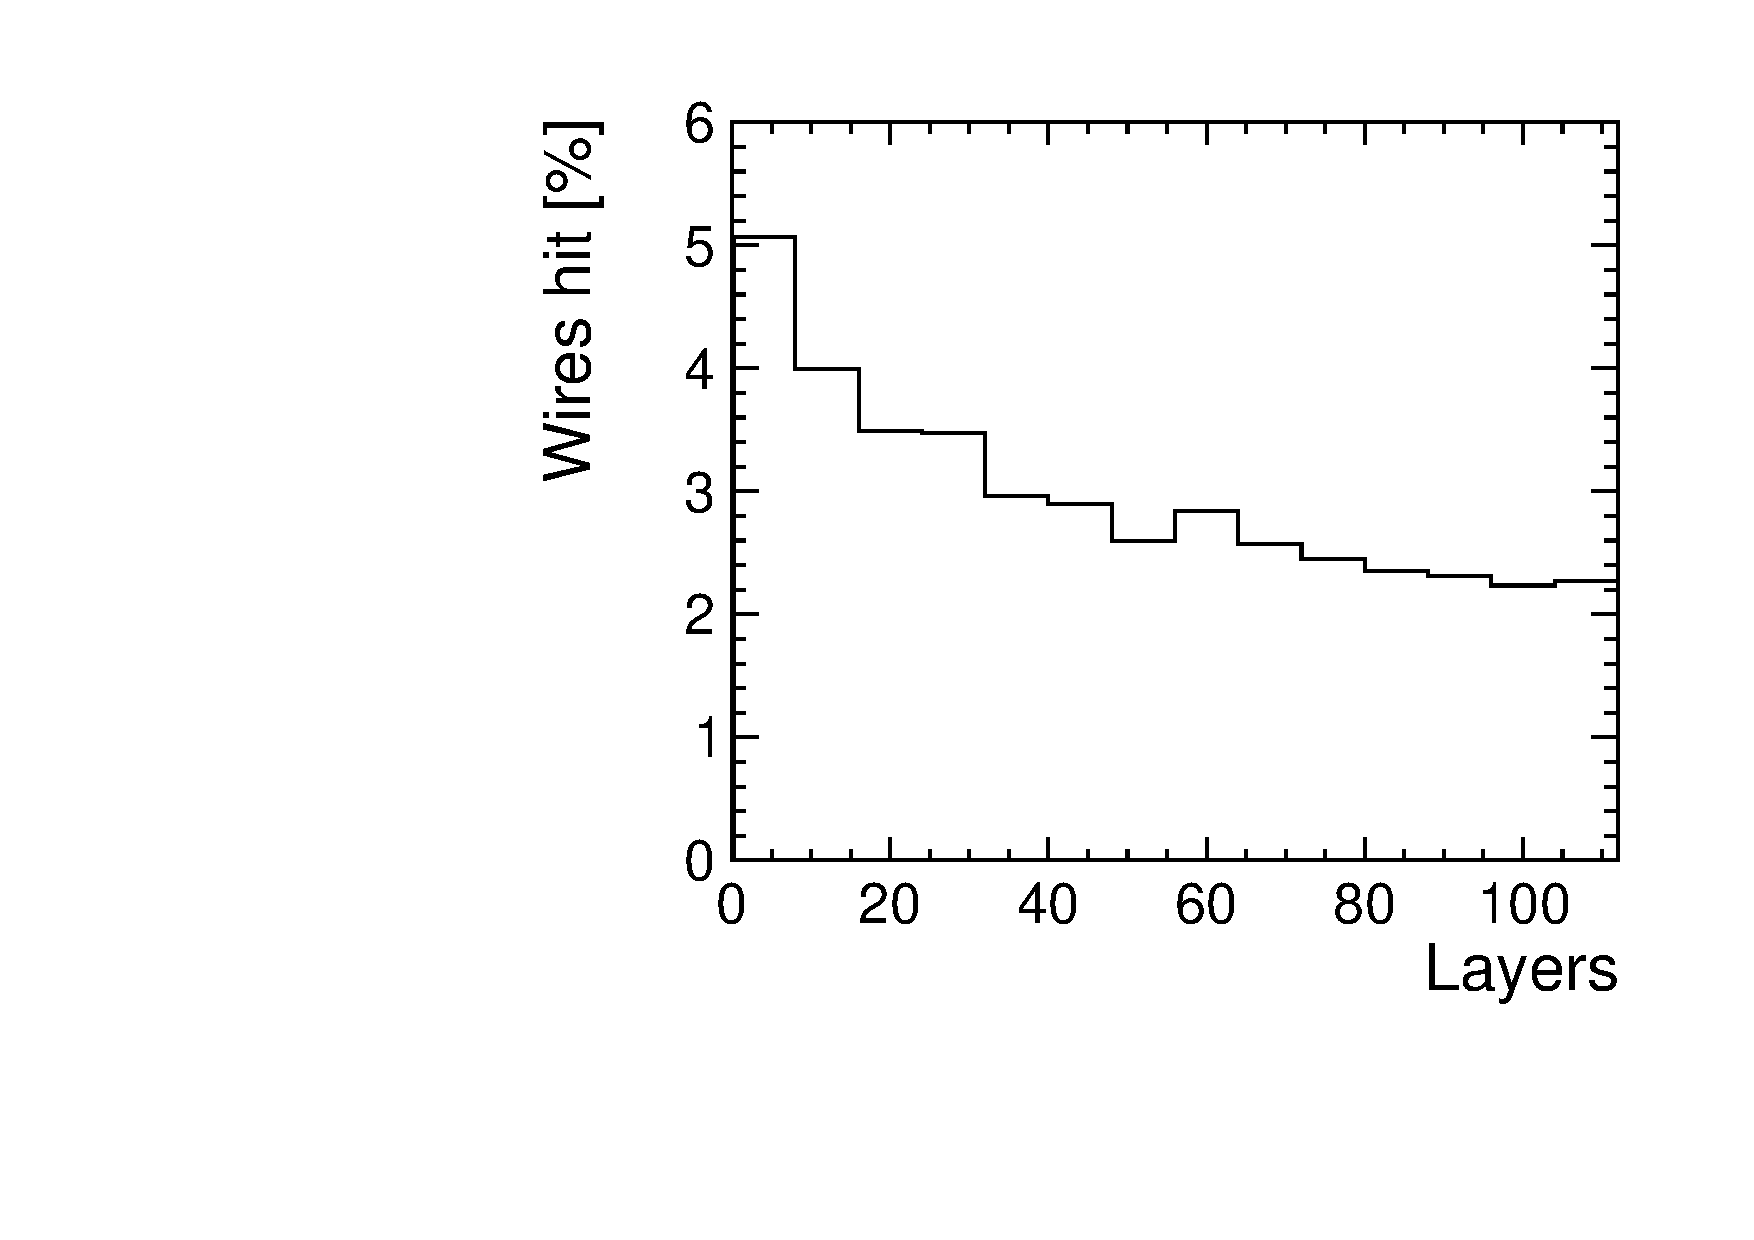
\includegraphics[width=\textwidth]{./figures/IPC_top.pdf}

      \begin{itemize}
        \item Average occupancy: 2.9\%
      \end{itemize}
    \end{block}

  \end{columns}

  \begin{itemize}
    \item The effect of this background does not pose problem for the track reconstruction.
  \end{itemize}

\end{frame}

%%%%%%%%%%%%%%%%%%%%%%%%%%%%%
%         SLIDE             %
%%%%%%%%%%%%%%%%%%%%%%%%%%%%%
\begin{frame}
	\frametitle{$\gamma\gamma\rightarrow$ hadrons}

  \begin{columns}
    \column{0.5\textwidth}
      \begin{block}{E\textsubscript{cm} = 91.2~GeV (Z stage)}
        \centering
        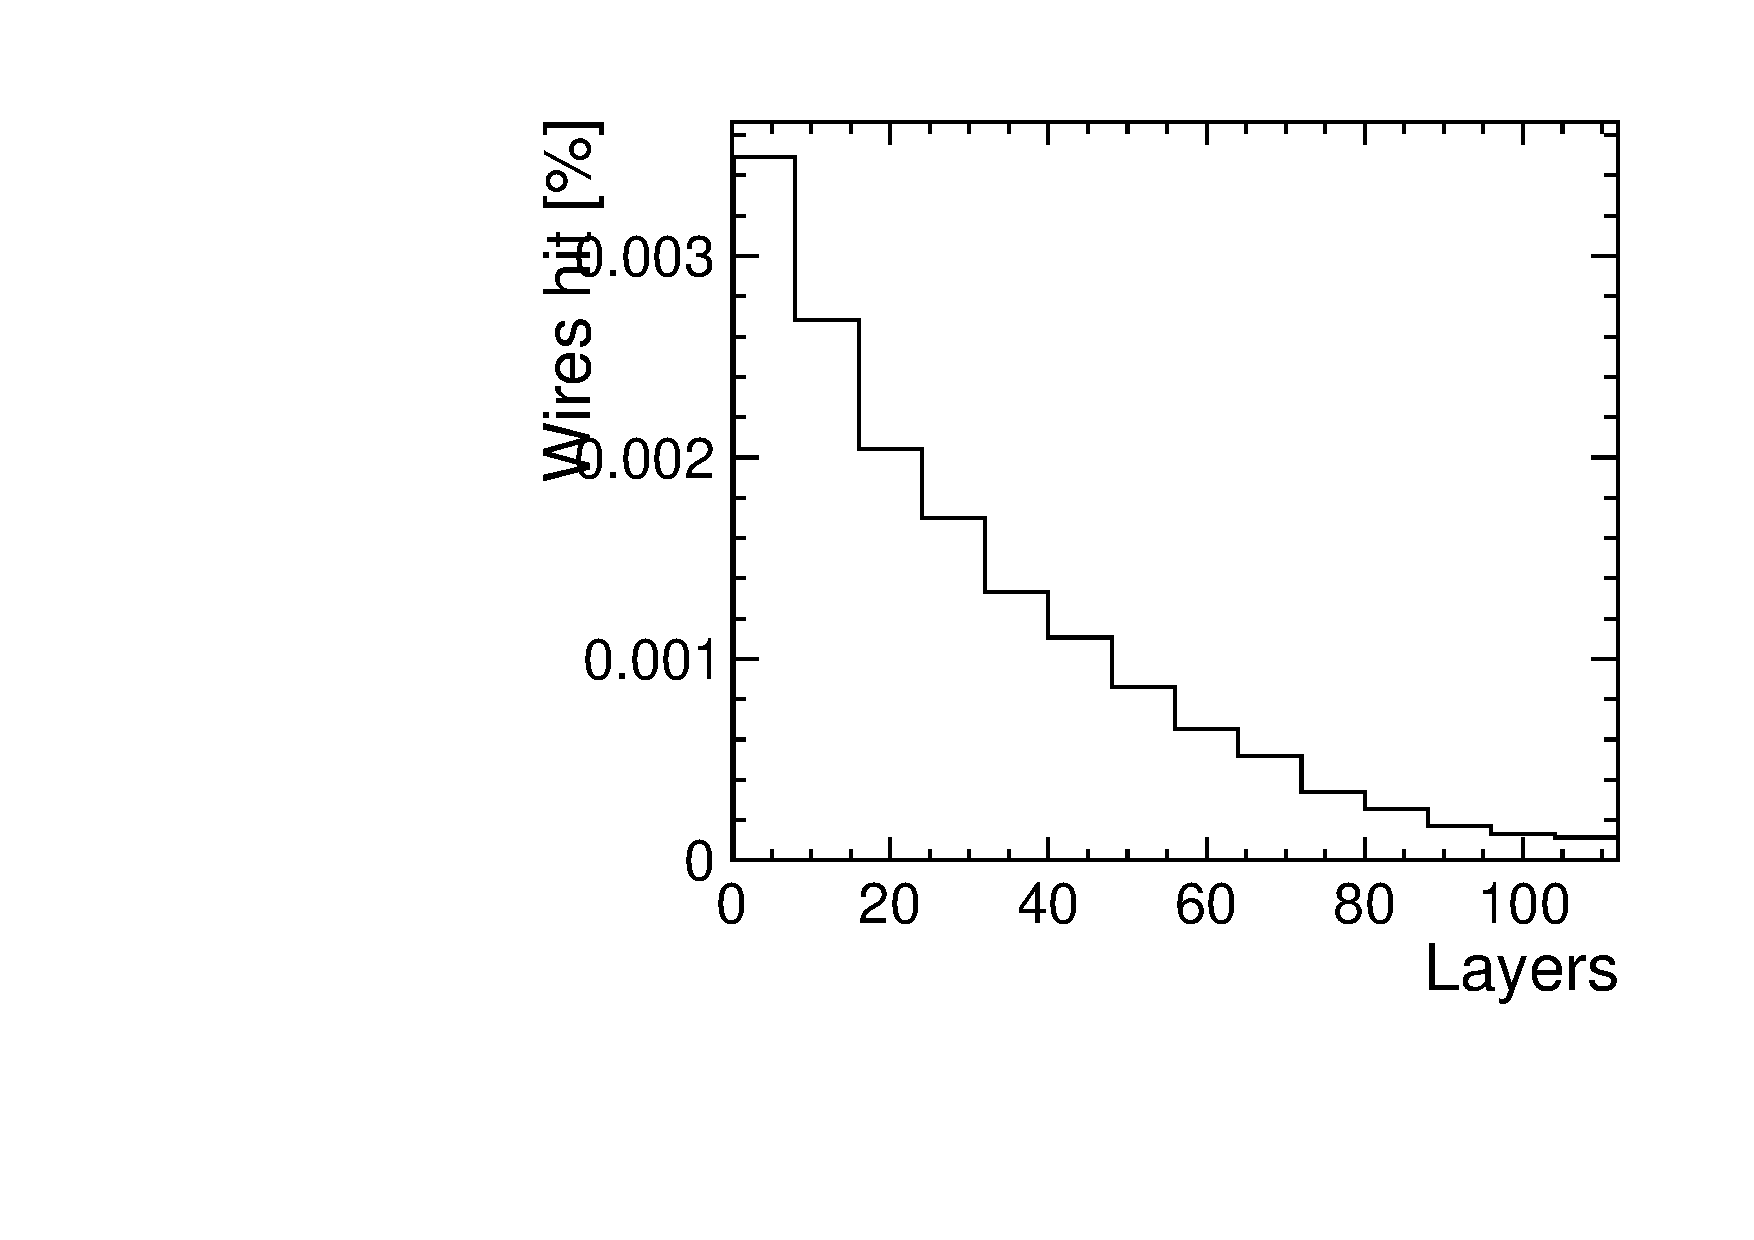
\includegraphics[width=\textwidth]{./figures/Hadrons_SL_Z.pdf}

        \begin{itemize}
          \item Average occupancy: 0.001\%
        \end{itemize}
      \end{block}

    \column{0.5\textwidth}
    \begin{block}{E\textsubscript{cm} = 365~GeV (top stage)}
      \centering
      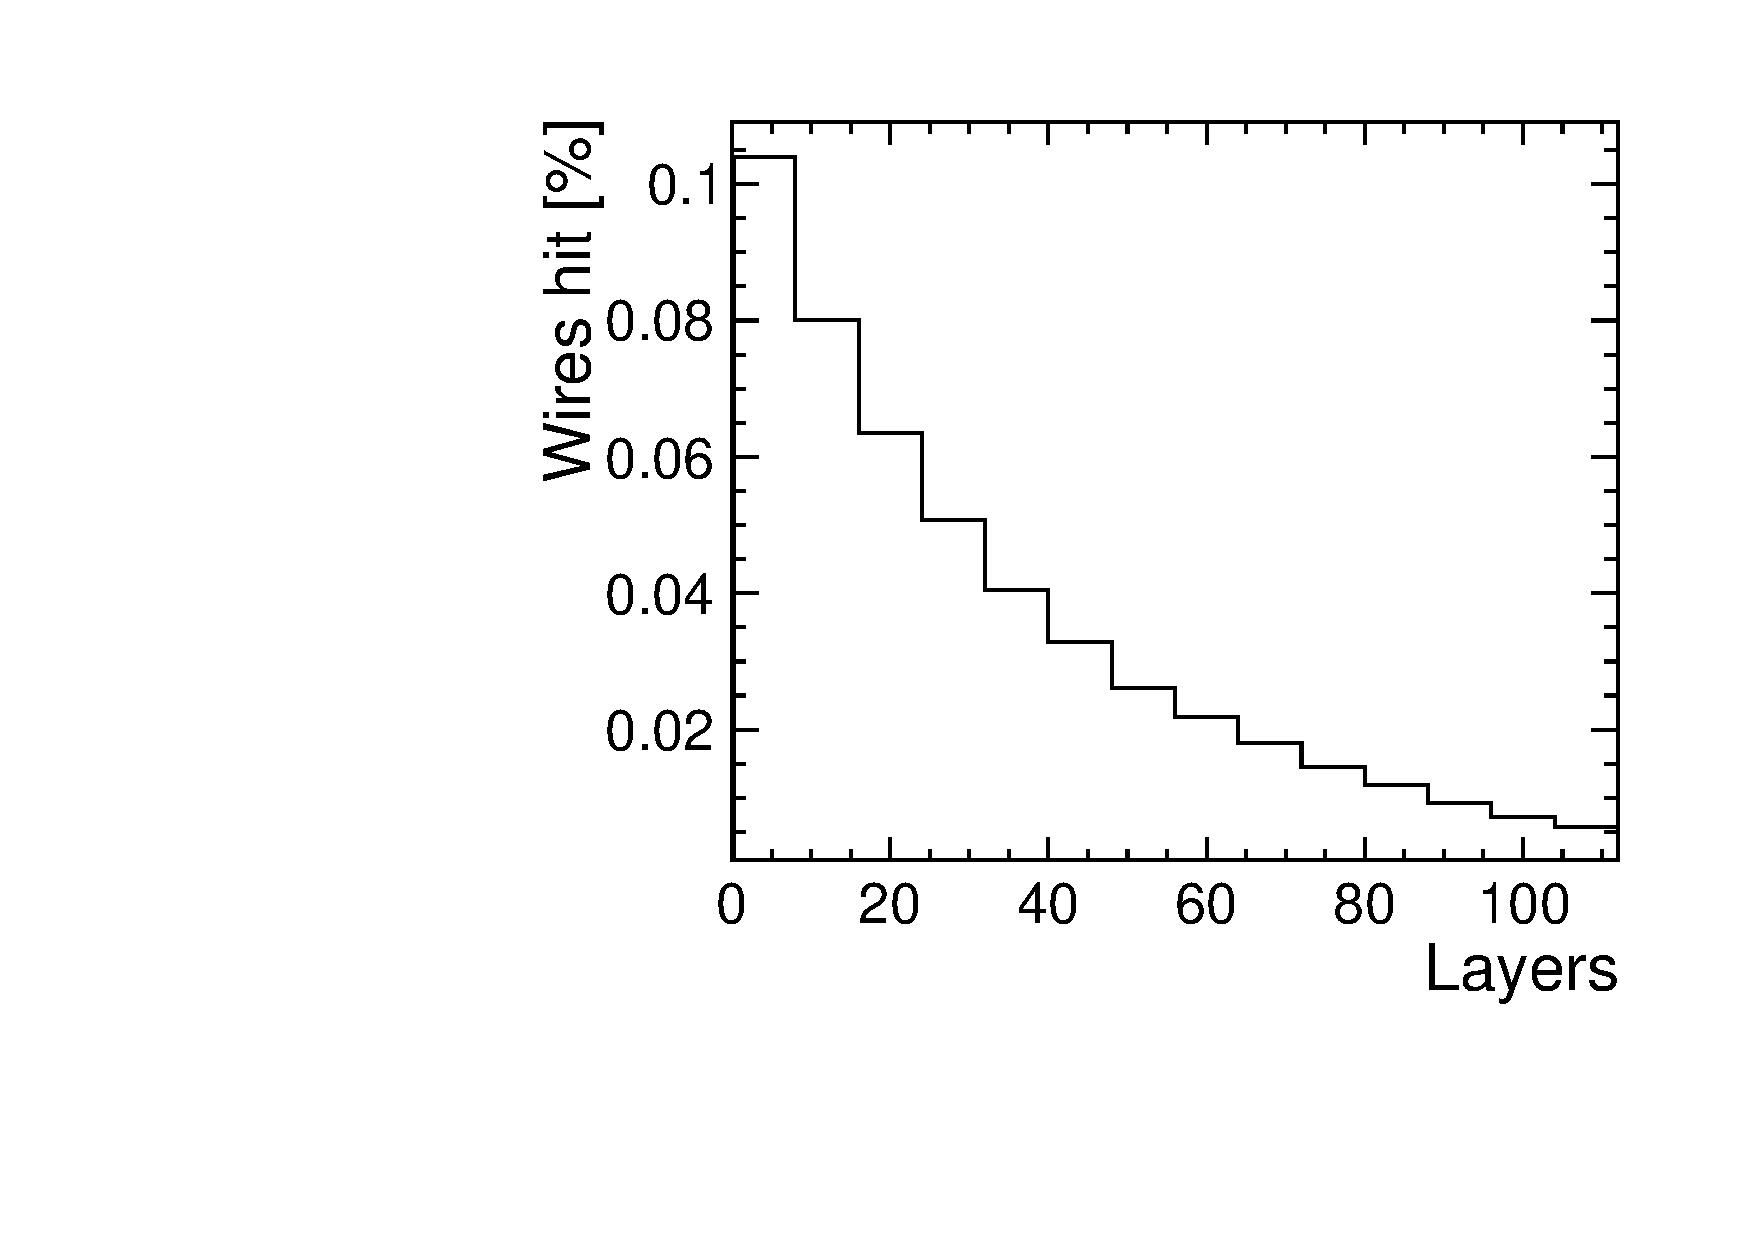
\includegraphics[width=\textwidth]{./figures/Hadrons_SL_Top.pdf}

      \begin{itemize}
        \item Average occupancy: 0.035\%
      \end{itemize}

    \end{block}
  \end{columns}

  \begin{itemize}
    \item Negligible effect
  \end{itemize}

\end{frame}

%%%%%%%%%%%%%%%%%%%%%%%%%%%%%
%         SLIDE             %
%%%%%%%%%%%%%%%%%%%%%%%%%%%%%
\begin{frame}
	\frametitle{Synchrotron radiation: E\textsubscript{cm} = 365~GeV}

  \begin{itemize}
    \item The shielding stops most of the SR photons.
    \item Average occupancy: 0.2\%
    \item Negligible effect
  \end{itemize}
  \centering
  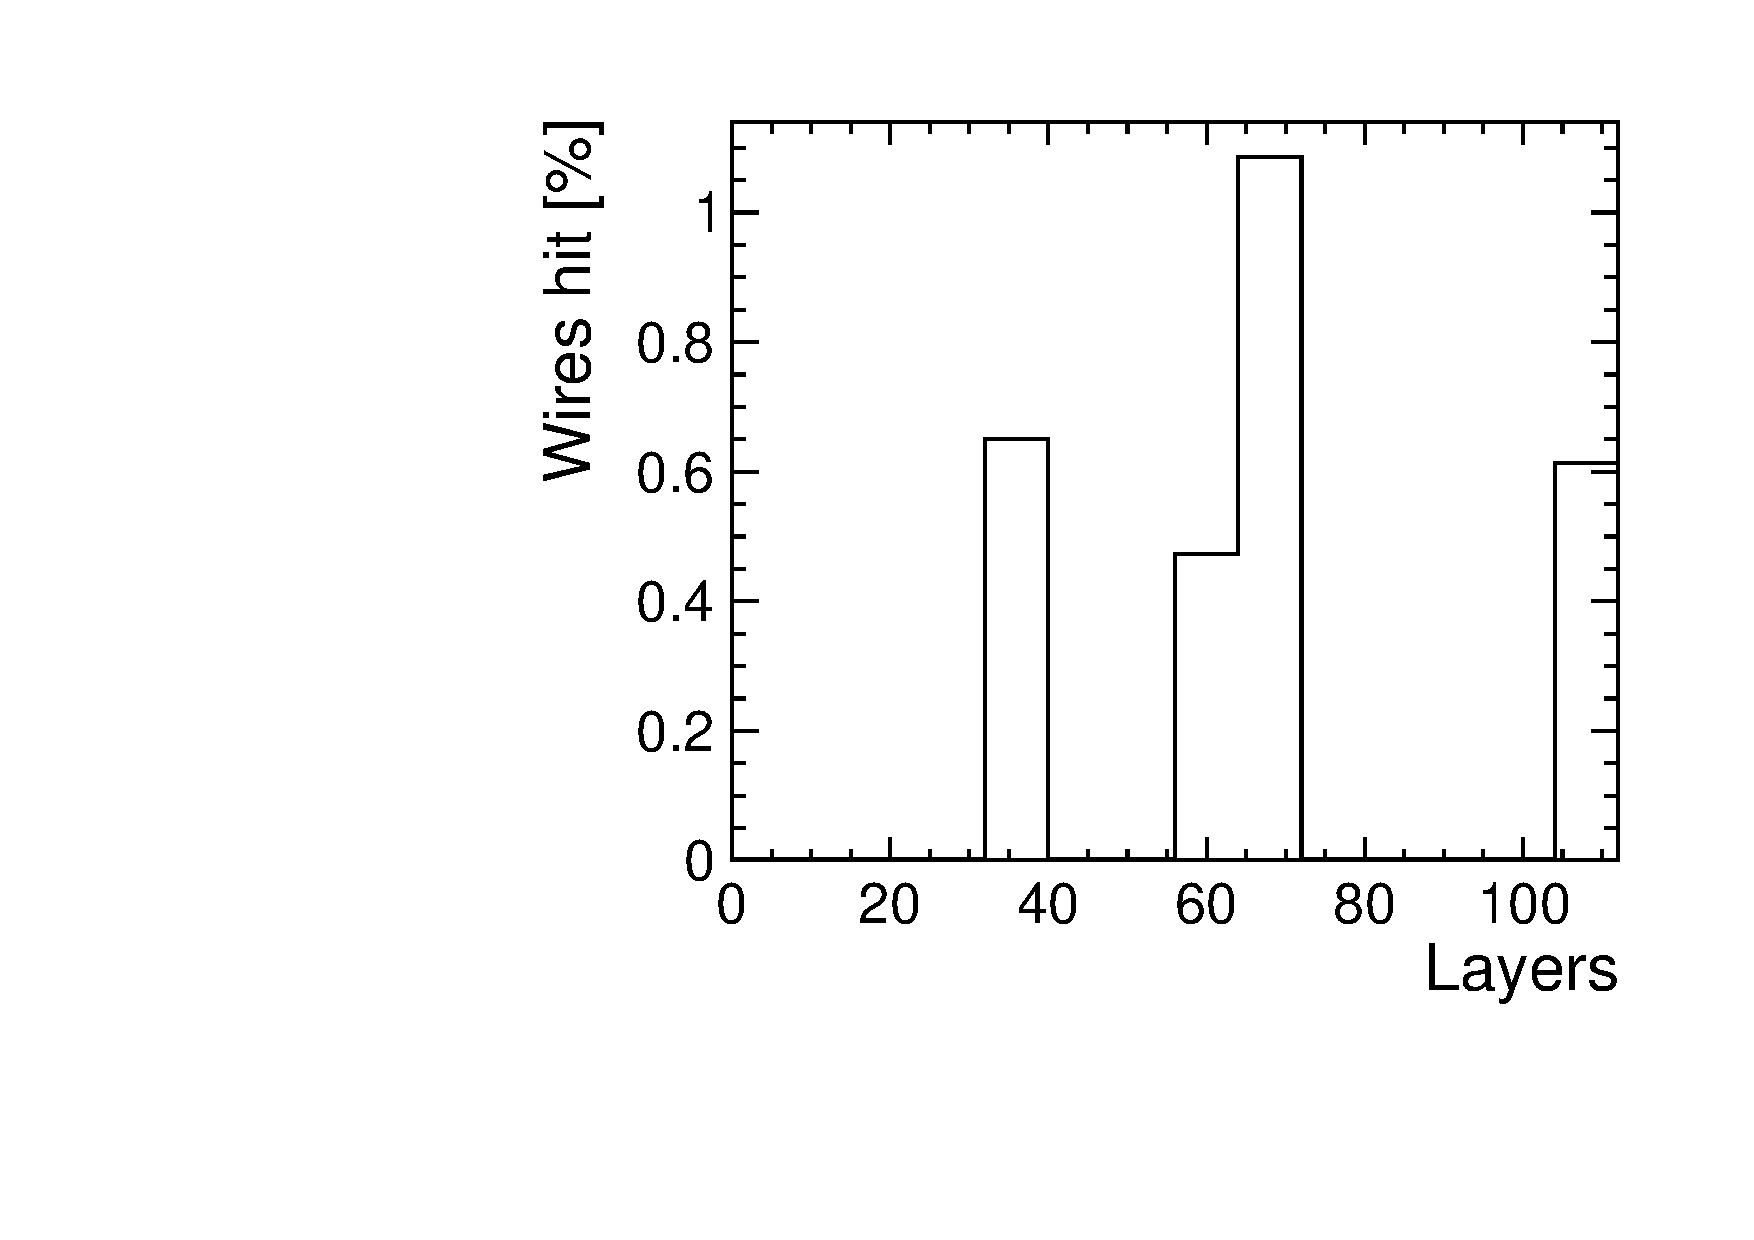
\includegraphics[width=0.5\textwidth]{./figures/SR_SL.pdf}

\end{frame}

%%%%%%%%%%%%%%%%%%%%%%%%%%%%%
%         SLIDE             %
%%%%%%%%%%%%%%%%%%%%%%%%%%%%%
\begin{frame}
	\frametitle{Summary: background occupancy in DCH}

  \begin{itemize}
    \item The overall effect of the backgrounds on the DCH remains small
    \item $e^+e^-$ pair background is the largest source of background
  \end{itemize}

  \vspace{0.5cm}

  \centering
  \begin{tabular}{l c c}
    \toprule
    Background & \multicolumn{2}{c}{Average occupancy} \\
     & E\textsubscript{cm} = 91.2~GeV &  E\textsubscript{cm} = 365~GeV \\
    \midrule
    $e^+e^-$ pair background & 1.1\% & 2.9\% \\
    $\gamma\gamma\rightarrow$hadrons & 0.001\% & 0.035\%  \\
    Synchrotron radiation & - & 0.2\% \\
    \bottomrule
  \end{tabular}
\end{frame}

%%%%%%%%%%%%%%%%%%%%%%%%%%%%%
%         SLIDE             %
%%%%%%%%%%%%%%%%%%%%%%%%%%%%%
\label{lastslide}
\begin{frame}
	\frametitle{Conclusions}

  \begin{itemize}
    \item The FCCSW is ready for the full simulation of the IDEA detector \vspace{0.5cm}
    \item Background estimations in full simulations have been performed for the drift chamber
    \begin{itemize}
      \item Low effect
    \end{itemize} \vspace{0.5cm}
    \item Contributions are more than welcome \\
    $\Rightarrow$ Input for tracking \\
    $\Rightarrow$ Dual-readout calorimeter, ...
  \end{itemize}

  \vspace{1cm}
  \Huge{Thank you for your attention!}
\end{frame}


%----------------------------------------------------------------------------------------
%	End of Document
%----------------------------------------------------------------------------------------
\end{document}
